\documentclass[12pt,a4paper]{article}
\usepackage[utf8]{inputenc}
\usepackage[ngerman]{babel}
\usepackage[T1]{fontenc}
\usepackage{amsmath}
\usepackage{amsfonts}
\usepackage{amssymb}
\usepackage{graphicx}
\usepackage{subfigure}
\author{Alexander Binsmaier, Manuel Mende, Yaroslav Direy}
\title{Auswertung MPGA -- günstige und ungünstige Parametrisierungen}

\begin{document}
\maketitle
\tableofcontents
\section{Allgemeines Vorgehen}
Um die Parametrisierung der Algorithmen gegeneinander auszuwerten, muss eine Vergleichsbasis geschaffen werden. Eine Möglichkeit ist es, den genetischen Multi-Populations-Algorithmus ohne Migration laufen zu lassen. Basierend auf den Ergebnissen dieses Durchlaufs können dann unterschiedliche Konfigurationen des Algorithmus ausgeführt und verglichen werden. Um die Komplexität zu relativieren, wurden einige Einschränkungen getroffen. Die Algorithmen sollen immer auf acht Chromosome umfassende Populationen angewendet werden. Die Parametrisierung des zugrunde liegenden genetischen Algorithmus ist identisch -- abgesehen von den verwendeten Fitnessfunktionen -- und die durchlaufenden Generationen werden auch konstant gehalten. Eine geeignete Anzahl Generationen wird durch die migrationslose Ausführung festgelegt. Als Variationsparameter verbleiben die Anzahl an Migrationen und die Anzahl an Generationen bis zur nächsten Migration. Zudem kann die Strategie variiert werden.
Primär existiert die uneingeschränkte Migration (unrestricted), bei der jede Population in jede andere Population migrieren kann. Als zweite Möglichkeit besteht die Ring-Migration. Hier wird semantisch nicht zusammenhängend in die nächste Population migriert. Die auf Nachbarschaft basierende Migrationsstrategie erlaubt eine Migration nur, wenn Ziel- und Quellpopulation auf der selben Seite -- also vor oder hinter -- der Parklücke liegen. 
Die Auswertung erfolgt im Anschluss und betrachtet vor allem die Entwicklung der mittleren Populationsfitness über die Epochen. Speziell gilt das Interesse, wie schnell ein akzeptables Fitness-Niveau erreicht wird. Auch die Testfälle der Ergebnispopulation werden entsprechend in die Bewertung mit eingehen, sowie deren Ähnlichkeit innerhalb der Populationen.

\section{Migrationsfreier Durchlauf}
Primär dient die migrationsfreie Ausführung des Algorithmus der Festlegung einer Vergleichsbasis. Zudem kann die Geschwindigkeit der Konvergenz des Algorithmus als Indiz für die Anzahl notwendiger Generationen für die migrierenden Ausführungen verwendet werden. Die Ausführung erfolgt dabei mit den selben Realisierungen der genetischen Algorithmen -- identische Fitnessfunktionen in den einzelnen Populationen, gleiche Parametrisierung der Rekombination und Mutation -- wie in den Durchläufen mit Migration. Um ein Generationslimit festzulegen, wir eine sehr hohe Anzahl Generationen gewählt. Für jede Population werden 5000 Epochen durchlaufen.

\subsection{Entwicklung der Fitness}
\begin{figure}
\centering
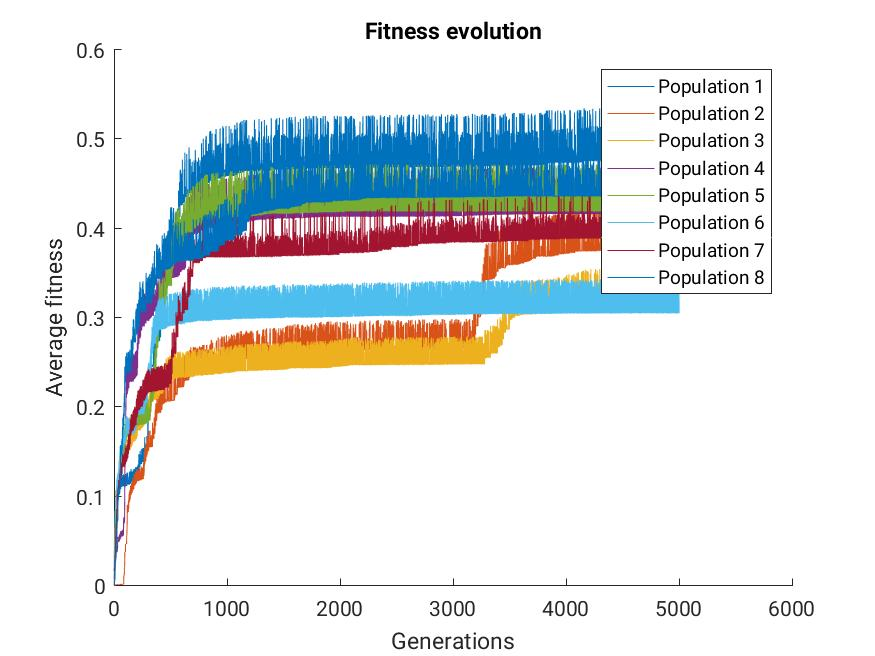
\includegraphics[width=.8\textwidth]{plain-fit.jpg}
\caption{Mittlere Fitness bei migrationsfreier Evolution}
\label{fig:plain_fit}
\end{figure}
Wie in Abbildung \ref{fig:plain_fit} ersichtlich, konvergiert die gemittelte Fitness der Populationen zu einem maximalen Wert von $0.6$, welcher für die beste Population bereits ab 1000 Generationen erreicht wird. Daher wurde als Generationslimit für die migrierenden Ausführungen 1000 Generationen gewählt. Zwar treten in einigen Generationen auch später noch Verbesserungen auf. Jedoch besteht die Hoffnung, dass ein migrierender Ansatz hier schneller zu besseren Werten führt.

\subsection{Testfälle}
Natürlich ist es erforderlich, dass die Fitness schnell konvergiert. Dennoch muss auch beachtet werden, dass die resultierenden Testfälle auch die Anforderungen erfüllen. Die Populationen wurden nach diversen Gesichtspunkten ausgewählt. So kann das Fahrzeug vor oder hinter der Parklücke liegen und tendenziell nach oben, unten, links oder rechts orientiert sein. Aus der Kombination von Lage und Orientierung ergeben sich acht Populationen, die jeweils charakteristische Chromosome hervorbringen. Diese müssen in der Ergebnispopulation auftreten.
\begin{figure}
\centering
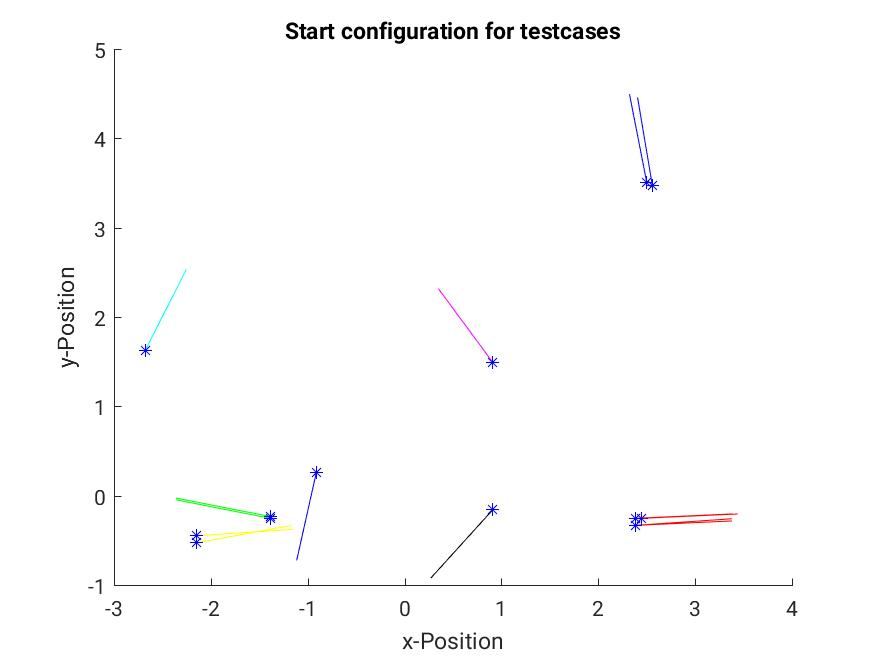
\includegraphics[width=.8\textwidth]{plain-tcs.jpg}
\caption{Ergebnispopulation ohne Migration (5000 Generationen)}
\label{fig:plain_tcs}
\end{figure}
Abbildung \ref{fig:plain_tcs} zeigt eine Ergebnispopulation ohne Migration. Deutlich sind die entsprechenden Klassen erkennbar.

\section{Schlechte Konfigurationen}
Seltene Migration vieler Chromosome führt zu Problemen.

\section{Gute Konfigurationen}
Häufige Migration weniger Chromosome liefert gute Ergebnisse.

\end{document}
